% cap2.tex

\chapter{Revisión Bibliográfica}
\label{ch:litRev} % la etiqueta para referencias

{\color{blue} En esta sección de debe incluir la revisión general y especifica de la investigación
desarrollada en la tesis.
Aparte de referencias antiguas, las citas deben incluir referencias sustanciales de
los 5 últimos años que den cuenta de la situación actual del tema a investigar,
evitar el uso de páginas web o fuentes no formales de información. (Máximo 15 páginas). }

\vspace{0.5cm}

Para citar bibliografía use \citeA{de_gregorio_macroeconomiteoriy_2007} o bien
\cite{de_gregorio_macroeconomiteoriy_2007}, dependiendo de la redacción.

Para referirse a tablas o a figuras use Tabla \ref{tab:nombreTabla} o Figura \ref{fig:nombreFigura},
y para acrónimos como \gls{latex} definirlos en el archivo core/glosario.tex

\section{Título primer sub-capítulo}

Los títulos de los subcapítulos se escriben con mayúscula y sin negritas.

La primera enumeración dentro de un texto se escribe con letras: a, b, c, etc.


\begin{enumerate}

\item primer item

\end{enumerate}


\begin{table}[]
\label{tab:nombreTabla}
\centering
\begin{tabular}{|l|l|l|l|l|l|}
\hline
Individuo & G\'enero & \ldots & Act6 & Act6 & Act8 \\ \hline
A         &        &     & 1    & 1    & 1    \\ \hline
B         &        &     & 0    & 1    &      \\ \hline
\end{tabular}
\caption{Título de la tabla}
\end{table}

\begin{figure}
\label{fig:nombreFigura}
\centering
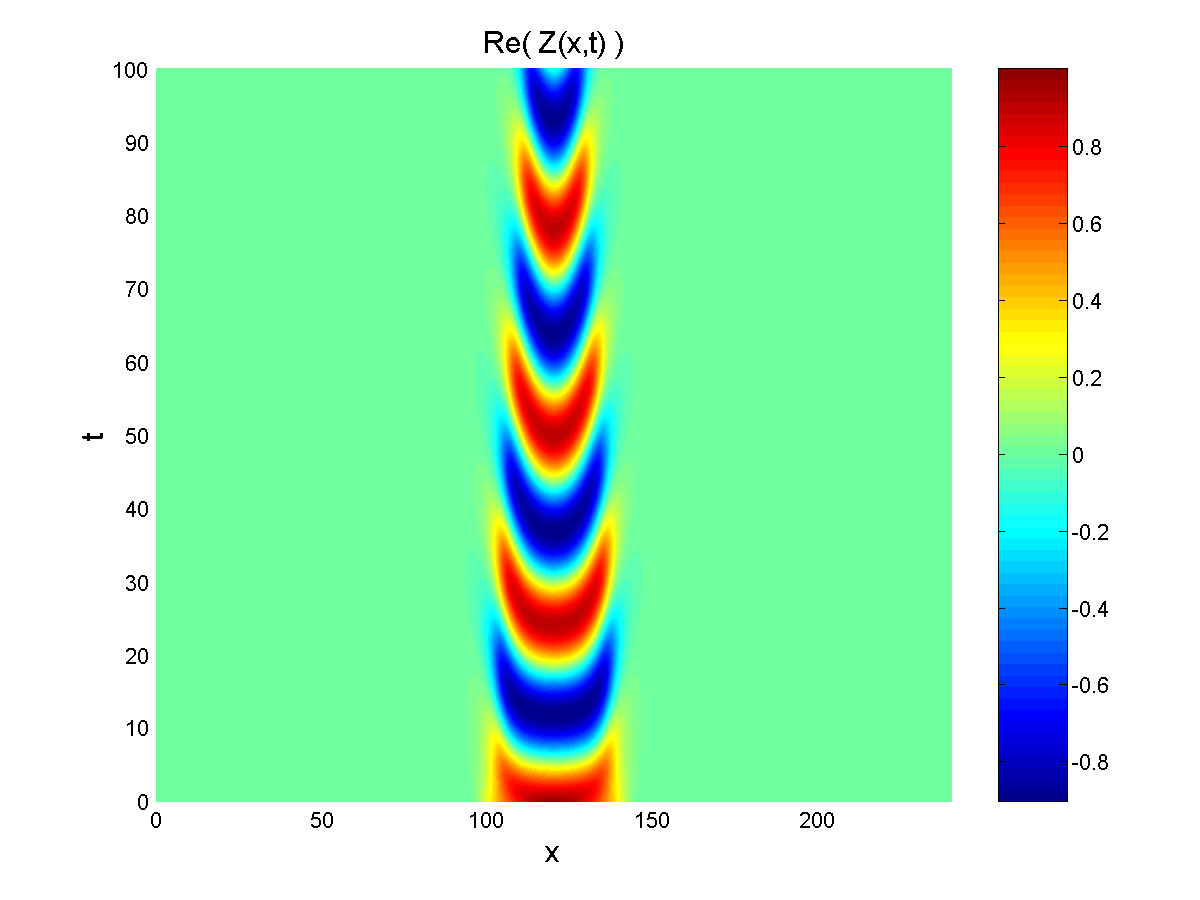
\includegraphics[scale=0.5]{images/cqgl_1}
\caption{Descripción de la figura.}
\end{figure}
